%% v8 - 11/23/2021

\documentclass{article}
\usepackage[margin=1in]{geometry}

\usepackage[tbtags]{amsmath}		% split tags on lower right
\usepackage{amssymb, mathrsfs}	% for math script fonts
\usepackage{physics}
\usepackage{graphicx}			% for images
\usepackage{tensor}				% for tensors
\usepackage{slashed}				% for Dirac slash
\usepackage{bm}					% for bold Greek
\usepackage[colorlinks=true]{hyperref}			% for hyperlinks in contents
\usepackage{cite}				% for citation numbering like 1--3 instead of 1, 2, 3
\usepackage{subcaption}
\usepackage[T1]{fontenc} 		% updated fonts (e.g. textcen has caps letters)
\usepackage{qcircuit}

\DeclareOldFontCommand{\rm}{\normalfont\rmfamily}{\mathrm}
\DeclareOldFontCommand{\sf}{\normalfont\sffamily}{\mathsf}
\DeclareOldFontCommand{\tt}{\normalfont\ttfamily}{\mathtt}
\DeclareOldFontCommand{\bf}{\normalfont\bfseries}{\mathbf}
\DeclareOldFontCommand{\it}{\normalfont\itshape}{\mathit}
\DeclareOldFontCommand{\sl}{\normalfont\slshape}{\@nomath\sl}
\DeclareOldFontCommand{\sc}{\normalfont\scshape}{\@nomath\sc}

%\setlength\parindent{0pt}

\let\no\nonumber
\let\cal\mathcal

\renewcommand{\epsilon}{\varepsilon}	% use varepsilon
\DeclareMathOperator{\diag}{diag}
\DeclareMathOperator{\sign}{sign}
\DeclareMathOperator{\QFT}{QFT}
\DeclareMathOperator{\lcm}{lcm}
\newcommand{\textcen}[1]{\centerline{\textbf{\textsc{#1}}}} 		% text dividing within a section
%\renewcommand\labelitemi{--} % for prettier bullet
\newcommand{\propbox}[1]{\noindent \fbox{ \parbox{\textwidth}{#1}}}		% box for propositions
\newcommand{\Mod}[1]{\ (\mathrm{mod}\ #1)}

\numberwithin{equation}{section} 		% number equations by section

\title{Quantum Computing}
\author{Kevin Chen}
\date{\today}

\begin{document}

\maketitle

\tableofcontents

\newpage
\section*{Foreword}
The purpose of these notes is mainly for personal reference, so the overall presentation will be very terse.
I hope this may also serve as a useful resource for others.
The primary reference is John Watrous's lecture notes, which can be found at \href{https://cs.uwaterloo.ca/~watrous/QC-notes/}{https://cs.uwaterloo.ca/~watrous/QC-notes/}.
This is supplemented in some places by John Preskill's lecture notes, which can be found at \href{http://theory.caltech.edu/~preskill/ph229/}{https://theory.caltech.edu/~preskill/ph229/}.

\newpage

%%%%%%%%%%%%%%%%%%%%%%%%%%%%%%%%%%%%%%%%%%%%%%%%%%%%%%%%%%%%%%%%%%%%%%%%%%%%%%%%
\section{Quantum mechanics} %%%%%%%%%%%%%%%%%%%%%%%%%%%%%%%%%%%%%%%%%%%%%%%%%%%%
\label{sec-qm} %%%%%%%%%%%%%%%%%%%%%%%%%%%%%%%%%%%%%%%%%%%%%%%%%%%%%%%%%%%%%%%%%
%%%%%%%%%%%%%%%%%%%%%%%%%%%%%%%%%%%%%%%%%%%%%%%%%%%%%%%%%%%%%%%%%%%%%%%%%%%%%%%%

We first review some basic facts about quantum mechanics that will be important in discussing quantum computing.
Knowledge of quantum mechanics and notation is assumed.

\begin{enumerate}
	\item A \textbf{qubit} is a state (i.e.~a vector) of a two-dimensional complex vector space. A general qubit $\ket{\psi}$ can be written as
		\begin{align} \label{eq-1-qubit}
			\ket{\psi} = \alpha \ket{0} + \beta \ket{1} ~,
		\end{align}
		where $\ket{0}$, $\ket{1}$ are the basis vectors and $\alpha$, $\beta$ are complex numbers.
		Note that the qubit is normalized:
		\begin{align}
			|\alpha|^2 + |\beta|^2 = 1 ~.
		\end{align}
	\item A system of two qubits is represented by taking the \emph{tensor product} of the qubits,
		\begin{align}
			(\alpha \ket{0} + \beta\ket{1}) \otimes (\gamma \ket{0} + \delta \ket{1}) =
			\mqty{ \phantom{+}\alpha \gamma \ket{0 0} \\ + \alpha \delta \ket{0 1} \\ + \beta \gamma \ket{1 0} \\ + \beta \delta \ket{1 1} } ~.
		\end{align}
		This implies that a system of $n$ qubits forms a state of a $2^n$-dimensional complex vector space.
		In what follows, we will often omit $\otimes$ and use the shorthand $\ket{0} \otimes \ket{1} \equiv \ket{0} \ket{1} \equiv \ket{01}$.
	\item The evolution of a system of qubits is represented by the application of a \emph{unitary operator},
		\begin{align}
			\ket{\Psi} \to U \ket{\Psi} ~,
		\end{align}
		where $U$ is a complex-valued matrix that satisfies
		\begin{align}
			U U^\dagger = U^\dagger U = I ~.
		\end{align}
	\item The measurement of a qubit yields one of two outcomes: $0$ or $1$.
		For the qubit described in (\ref{eq-1-qubit}), a measurement of $0$ occurs with probability $|\alpha|^2$ and a measurement of $1$ occurs with probability $|\beta|^2$.
		After the measurement, the qubit is altered and takes on the state corresponding to the measured outcome, either $\ket{0}$ or $\ket{1}$.
\end{enumerate}

Intuitively, a quantum computation is carried out by (i) preparing some input qubits, (ii) applying unitary operators to those qubits, and then (iii) measuring the result at the end.



%%%%%%%%%%%%%%%%%%%%%%%%%%%%%%%%%%%%%%%%%%%%%%%%%%%%%%%%%%%%%%%%%%%%%%%%%%%%%%%%
\section{Circuits} %%%%%%%%%%%%%%%%%%%%%%%%%%%%%%%%%%%%%%%%%%%%%%%%%%%%%%%%%%%%%
\label{sec-circuits} %%%%%%%%%%%%%%%%%%%%%%%%%%%%%%%%%%%%%%%%%%%%%%%%%%%%%%%%%%%
%%%%%%%%%%%%%%%%%%%%%%%%%%%%%%%%%%%%%%%%%%%%%%%%%%%%%%%%%%%%%%%%%%%%%%%%%%%%%%%%

In this section, we establish some common language to describe quantum algorithms, as well as explore some important consequences of quantum mechanics, such as quantum teleportation and no-cloning.

Let us define some useful unitary matrices:
\begin{align}
	X = \mqty( 0 & 1 \\ 1 & 0 ) ~, \qquad Y = \mqty( 0 & -i \\ i & 0 ) ~, \qquad Z = \mqty( 1 & 0 \\ 0 & -1 ) ~, \qquad H = \frac{1}{\sqrt{2}} \mqty(1 & 1 \\ 1 & -1) ~.
\end{align}
Note that $X$ is the NOT operator, i.e.~$\ket{0}$ is mapped to $\ket{1}$, and vice versa.
$H$ is called the \textbf{Hadamard matrix}.
All four matrices square to the identity matrix, $I$.

The circuit below shows the application of a unitary operator $U$ on the second qubit of a two-qubit system.
This is equivalent to the two-qubit unitary operator $I \otimes U$, which can be represented as a matrix on the ordered basis $\{\ket{00}, \ket{01}, \ket{10}, \ket{11}\}$,
\begin{gather}
	I \otimes U = \mqty( u_{00}&u_{01}&0&0 \\ u_{10}&u_{11}&0&0 \\ 0&0&u_{00}&u_{01} \\ 0&0&u_{10}&u_{11} ) ~. \\
	\no \\
	\Qcircuit @C=1.4em @R=1.2em {
		\lstick{\ket{\psi_1}} & \qw & \qw \\
		\lstick{\ket{\psi_2}} & \gate{U} & \qw \\
	}
\end{gather}

A qubit can control the application of a unitary operator on another qubit.
The circuit below shows the application of $U$ on the second qubit only when the first qubit is $\ket{1}$.
This two-qubit unitary operator is represented by the matrix,
\begin{gather}
	\mqty( 1&0&0&0 \\ 0&1&0&0 \\ 0&0&u_{00}&u_{01} \\ 0&0&u_{10}&u_{11} ) ~. \\
	\no \\
	\Qcircuit @C=1.4em @R=1.2em {
		\lstick{\ket{\psi_1}} & \ctrl{1} & \qw \\
		\lstick{\ket{\psi_2}} & \gate{U} & \qw \\
	}
\end{gather}

The \textbf{Bell states} are four mutually-orthogonal maximally entangled\footnote{A two-qubit state $\ket{\psi_{AB}}$ is \textbf{maximally entangled} when the partial trace of $\ket{\psi_{AB}} \bra{\psi_{AB}}$ over any one of the qubits is proportional to the identity matrix. Intuitively, a measurement on only one qubit acquires no information.} states,
\begin{align}
	\ket{\Phi^\pm} &= \frac{1}{\sqrt{2}} (\ket{00} \pm \ket{11} ) ~, \no \\
	\ket{\Psi^\pm} &= \frac{1}{\sqrt{2}} (\ket{01} \pm \ket{10} ) ~.
\end{align}
These states can be obtained from the basis states $\ket{00}, \ket{01}, \ket{10}, \ket{11}$ using the circuit,
\begin{gather} \label{eq-2-bell}
	\Qcircuit @C=1.4em @R=1.2em {
		\lstick{\ket{\psi_1}} & \gate{H} & \ctrl{1} & \qw \\
		\lstick{\ket{\psi_2}} & \qw & \gate{X} & \qw \\
	} \\
	\no \\
	\ket{00} \to \ket{\Phi^+} ~, \qquad
	\ket{01} \to \ket{\Psi^+} ~, \qquad
	\ket{10} \to \ket{\Phi^-} ~, \qquad
	\ket{11} \to \ket{\Psi^-} ~.
\end{gather}
We will now describe three phenomena related to entanglement.

\subsection{Dense coding}
\label{sec-circuits-dense}

Holveo's theorem states that the amount of classical information that can be retrieved from $n$ qubits is $n$ bits.
However, using entanglement, one can send two bits of classical information by sending only \emph{one} qubit.
\begin{itemize}
	\item Alice wants to send two bits of information to Bob.
	\item The state $\ket{\Phi^+}$ is created from two qubits $\ket{A}$ and $\ket{B}$. $\ket{A}$ is sent to Alice and $\ket{B}$ is sent to Bob.
	\item Alice prepares one of the four Bell states by applying single-qubit operators on $\ket{A}$:
		\begin{align}
			Z : \mqty{ \ket{\Phi^+} \leftrightarrow \ket{\Phi^-} ~, \\ \ket{\Psi^+} \leftrightarrow \ket{\Psi^-} ~, }  \qquad
			X : \mqty{ \ket{\Phi^+} \leftrightarrow \ket{\Psi^+} \phantom{-} ~, \\ \ket{\Phi^-} \leftrightarrow -\ket{\Psi^-} ~. }
		\end{align}
		Then Alice sends qubit $\ket{A}$ to Bob.
	\item Bob applies the circuit,
		\begin{align}
			\Qcircuit @C=1.4em @R=1.2em {
				\lstick{\ket{A}} & \ctrl{1} & \gate{H} & \qw \\
				\lstick{\ket{B}} & \gate{X} & \qw & \qw \\
			}
		\end{align}
		to undo the circuit in (\ref{eq-2-bell}) and map the four Bell states back to the basis states $\ket{00}, \ket{01}, \ket{10}, \ket{11}$.
		Bob can then perform measurements to determine which state he has and read off Alice's message.
\end{itemize}
This entire operation can be described by a circuit.
Suppose the two bits Alice wants to send are $ab$.
Double lines in the circuit represent classical bits, and the meter represents a measurement.
\begin{align}
	\Qcircuit @C=1.4em @R=1.2em {
		\lstick{a}&			\cw&			\cw&			\cctrl{2} \\
		\lstick{b}& 			\cw&			\cw&			\cw&			\cctrl{1} \\
		\lstick{\ket{0}}&	\gate{H}&	\ctrl{1}&	\gate{Z}&	\gate{X}&	\ctrl{1}&	\gate{H}&	\meter&	\rstick{a} \cw \\
		\lstick{\ket{0}}&	\qw&			\gate{X}&	\qw&			\qw&			\gate{X}&	\qw&			\meter&	\rstick{b} \cw \\
	}
\end{align}

\subsection{Teleportation}
\label{sec-circuits-tele}

Using entanglement, a qubit can be teleported by sending two bits of classical information.
\begin{itemize}
	\item Alice has a qubit $\ket{\psi}$ that she wants to give to Bob.
	\item The state $\ket{\Phi^+}$ is created from two qubits $\ket{A}$ and $\ket{B}$. $\ket{A}$ is sent to Alice and $\ket{B}$ is sent to Bob.
	\item If we let $\ket{\psi} = \alpha \ket{0} + \beta \ket{1}$, the state describing all three qubits is
		\begin{align}
			(\alpha \ket{0} + \beta \ket{1}) \frac{1}{\sqrt{2}} (\ket{00} + \ket{11}) = \frac{1}{\sqrt{2}} \qty( \alpha \ket{000} + \alpha \ket{011} + \beta \ket{100} + \beta \ket{111} ) ~.
		\end{align}
		Alice applies the circuit below on the two qubits $\ket{\psi}$, $\ket{A}$ in her possession:
		\begin{align}
			\Qcircuit @C=1.4em @R=1.2em {
				\lstick{\ket{\psi}} & \ctrl{1} & \gate{H} & \qw \\
				\lstick{\ket{A}} & \gate{X} & \qw & \qw \\
			}
		\end{align}
		The three-qubit state becomes
		\begin{align}
			\frac{1}{2} \qty\Big[ \ket{00}  (\alpha \ket{0} + \beta \ket{1}) + \ket{01} ( \beta \ket{0} + \alpha \ket{1} ) + \ket{10} (\alpha \ket{0} - \beta \ket{1} ) + \ket{11} (- \beta \ket{0} + \alpha \ket{1} ) ] ~.
		\end{align}
		Alice makes a measurement on her two qubits to obtain two classical bits $ab$, which she sends to Bob.
		This measurement causes qubit $\ket{B}$ to be one of four possibilities, depending on $ab$.
		The possibilities are tabulated below.
		\[ \begin{array}{r | l}
			ab & \ket{B} \\ \hline
			00 & \alpha \ket{0} + \beta \ket{1} \\
			01 & \beta \ket{0} + \alpha \ket{1} = X (\alpha \ket{0} + \beta \ket{1}) \\
			10 & \alpha \ket{0} - \beta \ket{1} = Z (\alpha \ket{0} + \beta \ket{1}) \\
			11 & - \beta \ket{0} + \alpha \ket{1} = XZ (\alpha \ket{0} + \beta \ket{1})
		\end{array} \]

	\item Given the bits $ab$, Bob knows exactly what state his qubit $\ket{B}$ is in.
	He can apply single-qubit operators on $\ket{B}$ to obtain the original state $\alpha \ket{0} + \beta \ket{1}$ that Alice had.
\end{itemize}

The circuit below describes this entire operation.
\begin{align}
	\Qcircuit @C=1.4em @R=1.2em {
		\lstick{\ket{\psi}}&	\qw&			\qw&			\ctrl{1}&	\gate{H}&	\meter&	\cw&			\cctrl{2} \\
		\lstick{\ket{0}}&	\gate{H}&	\ctrl{1}&	\gate{X}&	\qw&			\meter&	\cctrl{1} \\
		\lstick{\ket{0}}&	\qw&			\gate{X}&	\qw&			\qw&			\qw&		\gate{X}&	\gate{Z}&	\rstick{\ket{\psi}} \qw\\
	}
\end{align}

\subsection{No-cloning}
\label{sec-circuits-noclone}

Note that in teleportation, the original $\ket{\psi}$ qubit held by Alice is destroyed.
It is not possible to clone a qubit.
More precisely, there is no unitary operator that maps $\ket{\psi} \otimes \ket{0}$ to $\ket{\psi} \otimes \ket{\psi}$ for all qubits $\ket{\psi}$.

To prove this, let $\ket{\psi}$, $\ket{\phi}$ be two different qubits where $\braket{\psi}{\phi} \neq 0$.
\begin{align}
	\braket{\psi}{\phi} &= ( \bra{\psi} \otimes \bra{0} ) (\ket{\phi} \otimes \ket{0}) \no \\
	&= ( \bra{\psi} \otimes \bra{0} ) U^\dagger U (\ket{\phi} \otimes \ket{0} ) \no \\
	&= ( \bra{\psi} \otimes \bra{\psi} ) (\ket{\phi} \otimes \ket{\phi} ) \no \\
	&= \braket{\psi}{\phi}^2 ~.
\end{align}
This implies that $\braket{\psi}{\phi} = 1$, i.e.~they are the same qubit, which is a contradiction.



%%%%%%%%%%%%%%%%%%%%%%%%%%%%%%%%%%%%%%%%%%%%%%%%%%%%%%%%%%%%%%%%%%%%%%%%%%%%%%%%
\section{Algorithms} %%%%%%%%%%%%%%%%%%%%%%%%%%%%%%%%%%%%%%%%%%%%%%%%%%%%%%%%%%%
\label{sec-algo} %%%%%%%%%%%%%%%%%%%%%%%%%%%%%%%%%%%%%%%%%%%%%%%%%%%%%%%%%%%%%%%
%%%%%%%%%%%%%%%%%%%%%%%%%%%%%%%%%%%%%%%%%%%%%%%%%%%%%%%%%%%%%%%%%%%%%%%%%%%%%%%%

We will now describe some quantum algorithms that scale better than their classical counterparts.

\subsection{Deutsch's algorithm}
\label{sec-algo-deutsch}

\propbox{
	Given a function $f: \{0, 1\} \to \{0, 1\}$ on one bit, determine whether it is \textbf{constant} (i.e.~same output for all inputs) or \textbf{balanced} (i.e.~the number of inputs for which $f$ equals $0$ and $1$ are equal).
}\\

Classically, two queries of $f$ are needed to solve this problem.
Quantum mechanically, if we have access to the two-qubit operator,\footnote{$B_f$ is unitary because it is a permutation operator; the states $\ket{a} \ket{b}$ and $\ket{a} \ket{b \oplus f(a)}$ are mapped to each other under $B_f$. This will be so for any function $f$.}
\begin{align} \label{eq-3-Bf}
	B_f \ket{a} \ket{b} = \ket{a} \ket{b \oplus f(a)} ~,
\end{align}
where $\oplus$ is the XOR operator, then this problem can be solved in one query using the circuit,
\begin{align}
	\Qcircuit @C=1.4em @R=1.2em {
		\lstick{\ket{0}}&	\gate{H}&	\multigate{1}{B_f}&	\gate{H}&	\meter \\
		\lstick{\ket{1}}&	\gate{H}&	\ghost{B_f}&			\qw \\
	}
\end{align}
Let us track the two-qubit state through this circuit.
The initial state is $\ket{0}\ket{1}$.
The state after the initial Hadamard gates is
\begin{align}
	\frac{1}{\sqrt{2}} (\ket{0} + \ket{1}) \frac{1}{\sqrt{2}} (\ket{0} - \ket{1}) = \frac{1}{2} \ket{0} (\ket{0} - \ket{1}) + \frac{1}{2} \ket{1} (\ket{0} - \ket{1}) ~.
\end{align}
$B_f$ maps this state to
\begin{align}
	& \frac{1}{2} \ket{0} (\ket{0 \oplus f(0)} - \ket{1 \oplus f(0)}) + \frac{1}{2} \ket{1} (\ket{0\oplus f(1)} - \ket{1 \oplus f(1)}) \no \\
	& \qquad = \frac{1}{2} (-1)^{f(0)} \ket{0} (\ket{0} - \ket{1}) + \frac{1}{2} (-1)^{f(1)} \ket{1} (\ket{0} - \ket{1}) \no \\
	& \qquad = \frac{1}{\sqrt{2}} \qty\big( (-1)^{f(0)} \ket{0} + (-1)^{f(1)} \ket{1}) \frac{1}{\sqrt{2}} (\ket{0} - \ket{1}) ~.
\end{align}
Note that the second qubit is independent of $f$ and always equals $H\ket{1}$.
This qubit is discarded in the computation.
Applying a final Hadamard gate to the first qubit gives us the state $(-1)^{f(0)} \ket{f(0) \oplus f(1)}$.
A measurement of this state determines whether $f(0) \oplus f(1) = 0$ (constant) or $= 1$ (balanced).

\subsection{Deutsch-Jozsa algorithm}
\label{sec-algo-dj}

\propbox{
	Given a function $f: \{0, 1\}^n \to \{0, 1\}$ on $n$ bits, determine whether it is constant or balanced.
	$f$ is guaranteed to be one of these two cases.
}\\

This is a generalization of Deutsch's problem.
Classically, up to $2^{n-1}+1$ queries are needed to solve this problem in the worst-case scenario.
Probabilistically, with $k$ queries we can solve this problem with a probability of error $\leq 2^{1-k}$ by guessing ``constant'' when all $k$ outputs are equal.
Quantum mechanically, if we have access to the $(n+1)$-qubit operator $B_f$, which is defined in the same way as in (\ref{eq-3-Bf}) where $a$ represents an $n$-bit vector, then this problem can be solved in one query using the circuit,
\begin{align}
	\Qcircuit @C=1.4em @R=1.2em {
		\lstick{\ket{0}_1}&	\gate{H}&	\multigate{3}{B_f}&	\gate{H}&	\meter \\
		\vdots&				& 			& 					\vdots \\
		\lstick{\ket{0}_n}&	\gate{H}&	\ghost{B_f}&			\gate{H}&	\meter \\
		\lstick{\ket{1}}&	\gate{H}&	\ghost{B_f}&			\qw \\
	}
\end{align}
Let us track the state through this circuit.
The state after the initial Hadamard gates is
\begin{align}
	\frac{1}{2^{n/2}} \sum_{x \in \{0, 1\}^n} \ket{x} \frac{1}{\sqrt{2}} (\ket{0} - \ket{1}) ~.
\end{align}
$B_f$ maps this to
\begin{align}
	\frac{1}{2^{n/2}} \sum_{x \in \{0, 1\}^n} (-1)^{f(x)}\ket{x} \frac{1}{\sqrt{2}} (\ket{0} - \ket{1}) ~.
\end{align}
Discarding the final qubit and operating the final Hadamard gates, we have
\begin{align}
	\frac{1}{2^{n/2}} \sum_{x \in \{0, 1\}^n} (-1)^{f(x)} H^{\otimes n} \ket{x}
	& = \frac{1}{2^{n/2}} \sum_{x \in \{0, 1\}^n} (-1)^{f(x)} \qty( \frac{1}{2^{n/2}} \sum_{y \in \{0, 1\}^n} (-1)^{x \cdot y} \ket{y} ) \no \\
	& = \sum_{y \in \{0, 1\}^n} \qty( \frac{1}{2^n} \sum_{x \in \{0, 1\}^n} (-1)^{f(x) + x \cdot y} ) \ket{y} ~,
\end{align}
where $x \cdot y$ is interpreted as the dot product of two $n$-bit vectors $x$ and $y$, taken modulo 2.
Note that the amplitude for the $\ket{y} = \ket{0^n}$ state simplifies when $f$ is constant or balanced:
\begin{align}
	\frac{1}{2^n} \sum_{x \in \{0, 1\}^n} (-1)^{f(x)} = \begin{cases} (-1)^{f(0)} & \text{if $f$ is constant,} \\ 0 & \text{if $f$ is balanced.} \end{cases}
\end{align}
Therefore a measurement of the $n$ output qubits produces an $n$-bit vector, which are all 0 only when $f$ is constant.
Otherwise, $f$ is balanced.

\subsection{Bernstein-Vazirani algorithm}
\label{sec-algo-bv}

\propbox{
	Given a function $f: \{0, 1\}^n \to \{0, 1\}$ defined by
	\begin{align*}
		f(x) = x \cdot s ~,
	\end{align*}
	where $s$ is a secret $n$-bit vector, determine $s$.
}\\

This is a variation on the Deutsch-Jozsa problem, since when $s \neq 0$ iff the function $f$ is balanced.
Classically, $n$ queries are needed to solve this problem.
Quantum mechanically, this problem can be solved in one query using the same circuit as for the Deutsch-Jozsa algorithm.
In the last step, the final state is
\begin{align}
	\sum_{y \in \{0, 1\}^n} \qty( \frac{1}{2^n} \sum_{x \in \{0, 1\}^n} (-1)^{x \cdot (s + y)} ) \ket{y}
\end{align}
The amplitude is non-zero only for $\ket{y} = \ket{s}$.
Therefore, a measurement of the $n$ output qubits produces the $n$-bit vector $s$.

This is the first problem that we have discussed so far for which the quantum algorithm, which requires $\order{1}$ queries, is faster than the probabilistic/classical algorithm, which requires $\order{n}$ queries.

\subsection{Simon's algorithm}
\label{sec-algo-simon}

\propbox{
	Given a function $f: \{0, 1\}^n \to \{0, 1\}^n$ that has a \textbf{period} $s$, i.e.
	\begin{align*}
		y = x \oplus s \quad\iff\quad f(y) = f(x) ~,
	\end{align*}
	determine $s$.
	Here $x$, $y$, and $s$ are all $n$-bit vectors and the operation $\oplus$ is taken element-wise.
}\\

Classically, this problem requires exponentially many queries to solve, even for a probabilistic solution---intuitively, the reason why is that the chance that two random inputs create the same output is $2^{-n}$.
Quantum mechanically, this problem can be solved in $\order{n}$ queries of the $2n$-qubit operator $B_f$ given in (\ref{eq-3-Bf}), where $a$ and $b$ both represent $n$-bit vectors.
Consider the following circuit:
\begin{align}
	\Qcircuit @C=1.4em @R=1.2em {
		\lstick{\ket{0}_1}&	\gate{H}&	\multigate{5}{B_f}&	\gate{H}&	\meter \\
		\vdots&				& 			& 					\vdots \\
		\lstick{\ket{0}_n}&	\gate{H}&	\ghost{B_f}&			\gate{H}&	\meter \\
		\lstick{\ket{0}_1}&	\qw&			\ghost{B_f}&			\qw&			\qw \\
		\vdots&				& 			& 					\vdots \\
		\lstick{\ket{0}_n}&	\qw&			\ghost{B_f}&			\qw&			\qw \\
	}
\end{align}
Let us track the state through this circuit.
The state after the initial Hadamard gates is
\begin{align}
	\frac{1}{2^{n/2}} \sum_{x \in \{0, 1\}^n} \ket{x} \ket{0^n} ~.
\end{align}
$B_f$ maps this to
\begin{align}
	\frac{1}{2^{n/2}} \sum_{x \in \{0, 1\}^n} \ket{x} \ket{f(x)} ~.
\end{align}
The state after the final Hadamard gates is
\begin{align}
	\frac{1}{2^{n/2}} \sum_{x \in \{0, 1\}^n} H^{\otimes n} \ket{x} \ket{f(x)}
	& = \frac{1}{2^{n/2}} \sum_{x \in \{0, 1\}^n} \qty( \frac{1}{2^{n/2}} \sum_{y \in \{0, 1\}^n} (-1)^{x \cdot y} \ket{y} ) \ket{f(x)} \no \\
	& = \sum_{y \in \{0, 1\}^n} \ket{y} \qty( \frac{1}{2^n} \sum_{x \in \{0, 1\}^n} (-1)^{x \cdot y} \ket{f(x)} ) ~.
\end{align}

If $s = 0$, then $f$ is a bijective function and the term inside the parentheses is a sum over $2^n$ distinct states with coefficients that are either $\pm 2^{-n}$.
Therefore, the measurement of $y$ gives a random $n$-bit vector with uniform probability.

If $s \neq 0$, then $f$ is a two-to-one function.
Let $X \subset \{0, 1\}^n$ be a maximal set on which $f$ is bijective.
In other words, for each pair $x$ and $x \oplus s$ that map to the same output $f(x)$, $X$ contains exactly one element of the pair.
Then,
\begin{align}
	\frac{1}{2^n} \sum_{x \in \{0, 1\}^n} (-1)^{x \cdot y} \ket{f(x)} &= \frac{1}{2^n} \sum_{x \in X} \qty[ (-1)^{x \cdot y} \ket{f(x)} + (-1)^{(x + s) \cdot y} \ket{f(x+s)} ] \no \\
	&= \frac{1}{2^{n-1}}  \sum_{x \in X} (-1)^{x \cdot y} \qty[ \frac{1 + (-1)^{s \cdot y} }{2} ] \ket{f(x)}
\end{align}
For $y$ that satisfy $s \cdot y = 0$, this is a sum over $2^{n-1}$ distinct states with coefficients that are either $\pm 2^{-(n-1)}$.
Otherwise, the coefficient is zero when $s \cdot y \neq 0$.
Therefore, the measurement of $y$ gives a random $n$-bit vector that satisfies $s \cdot y = 0$ with uniform probability.

The strategy is to run this circuit until we collect $n-1$ linearly independent measurements $y_1, \dotsc, y_{n-1}$.
This will be very quick, since if we already have $k$ linearly independent vectors, the probability of obtaining a new linearly independent vector (if one exists) is $1 - 2^{k-n} \geq 50\%$.
The solution to the linear system of equations $s \cdot y_i = 0$ for $i = 1, \dotsc, n-1$ gives a unique non-zero vector $\hat{s}$.
Next, we run the circuit a couple more times to make sure there is not an $n$th linearly independent vector $y_n$.
If we do find $y_n$, then we conclude $s = 0$.
Otherwise, we conclude $s = \hat{s}$.
Since the probability of finding $y_n$, if it exists, is $50\%$, with $k$ more runs the probability of an incorrect conclusion is $2^{-k}$.
Thus we can find the period in $\order{n}$ queries with an arbitrarily low probability of error.

\subsection{Grover's algorithm}
\label{sec-algo-grover}

\propbox{
	Given a function $f: \{0, 1\}^n \to \{0, 1\}$, find an $x$ such that $f(x) = 1$, if such a $x$ exists.
}\\

Classically, $2^n$ queries are needed to solve this problem in the worst-case scenario.
Probabilistically, we still need $\order{2^n}$ queries for any finite probability of success.
Quantum mechanically,  this problem can be solved in $\order{2^{n/2}}$ queries of the $(n+1)$-qubit operator $B_f$, which is defined in the same way as in (\ref{eq-3-Bf}) where $a$ represents an $n$-bit vector.
Using $B_f$, we can implement the $n$-qubit operator,
\begin{align}
	Z_f : \ket{x} \mapsto (-1)^{f(x)} \ket{x} ~,
\end{align}
using a circuit similar to the one used for the Deutch-Josza algorithm:
\begin{align}
	\Qcircuit @C=1.4em @R=1.2em {
		\lstick{\ket{x}}&	\qw& 		\multigate{1}{B_f}& 	\qw& 		\rstick{(-1)^{f(x)} \ket{x}} \qw \\
		\lstick{\ket{1}}&	\gate{H}&	\ghost{B_f}&			\gate{H}& 	\rstick{\ket{1}} \qw \\
	}
\end{align}
Note that $Z_f$ can be viewed as a reflection that flips any ``good vector'' $\ket{a} \mapsto - \ket{a}$, where $f(a) = 1$, and leaves ``bad vectors'' $\ket{b}$ unchanged, where $f(b) = 0$.
Let $A$ be the set of ``good vectors'' and $B$ be the set of ``bad vectors''.
We can alternatively write
\begin{align}
	Z_f = I - \sum_{a \in A} 2 \ket{a} \bra{a} = \sum_{b \in B} 2 \ket{b} \bra{b} - I ~.
\end{align}
Next, we define another $n$-qubit operator,
\begin{align}
	Z_h = 2 \ket{h} \bra{h} - I ~, \qquad \ket{h} \equiv \frac{1}{2^{n/2}} \sum_{x \in \{0, 1\}^n} \ket{x} ~,
\end{align}
which represents a reflection preserving the component parallel to $\ket{h}$.
This operator can be efficiently implemented by $Z_h = H^{\otimes n} Z_0 H^{\otimes n}$ where $Z_0 = 2 \ket{0}^n \bra{0}^n - I$ is negative the $n$-qubit operator that sends $\ket{0^n} \mapsto - \ket{0^n}$ but leaves all other vectors unchanged.

To summarize, $Z_f$ is a reflection that preserves the component parallel to the hyperplane spanned by $B$, and $Z_h$ is a reflection that preserves the component parallel to $\ket{h}$.
Let us define the normalized vectors,
\begin{align}
	\ket{A} = \frac{1}{\sqrt{|A|}} \sum_{a \in A} \ket{a} ~, \qquad
	\ket{B} = \frac{1}{\sqrt{|B|}} \sum_{b \in B} \ket{b} ~.
\end{align}
$\ket{h}$ is a (real) linear combination of $\ket{A}$ and $\ket{B}$.
On the (real) two-dimensional subspace spanned by $\{\ket{A}, \ket{B}\}$, the composition of two reflections $G = Z_h Z_f$ is a rotation through an angle $2\theta$, where $\theta$ is the acute angle between $\ket{h}$ and $\ket{B}$:
\begin{align}
	 \cos\theta = \braket{h}{B} = \frac{\sqrt{|B|}}{2^{n/2}} \quad\implies\quad \sin \theta = \frac{\sqrt{|A|}}{2^{n/2}} ~.
\end{align}
This is sketched below.
By repeatedly applying $G$ on the vector $\ket{\psi} = \ket{h}$, the resulting vector will eventually be almost parallel to $\ket{A}$.
A measurement at that time will have a high probability of yielding an element of $A$, that is, an $n$-bit vector that solves the problem.

\centerline{
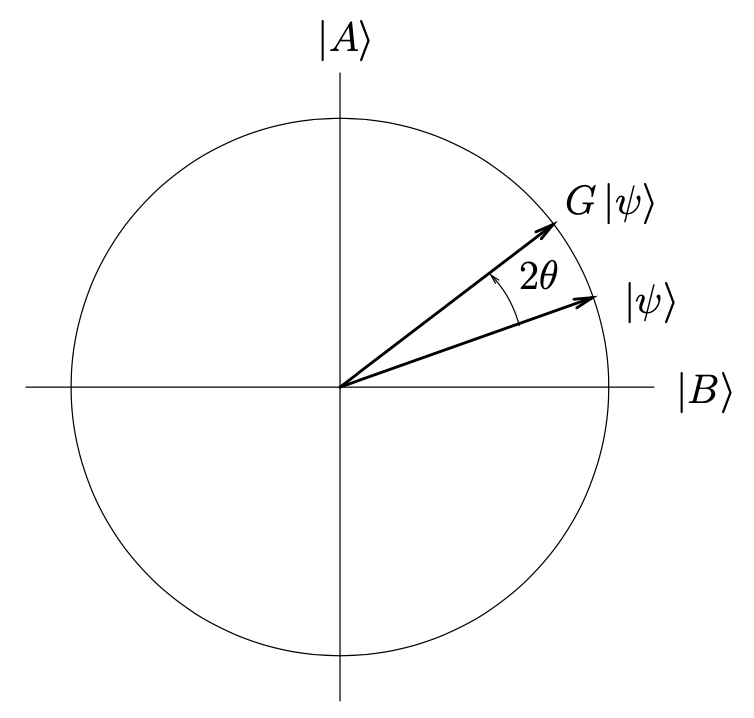
\includegraphics[width=5cm]{grover.png}
}

To be concrete, let us consider the case where $|A| = 1$.
After $k$ iterations of $G$ on $\ket{h} = \cos\theta \ket{A} + \sin\theta \ket{B}$, the state is
\begin{align}
	G^k \ket{h} = \cos[(2k+1)\theta] \ket{A} + \sin[(2k + 1)\theta] \ket{B} ~.
\end{align}
Thus, we should pick $k \approx  \pi / 4\theta - 1/2$ to maximize the amplitude of $\ket{A}$.
We can always pick a $k$ such that the amplitude of $\ket{B}$ is less than $\sin \theta$.
Taking a measurement, the probability of erroneously obtaining an element of $B$ is $ \leq 2^{-n}$.
To summarize Grover's algorithm,
\begin{itemize}
	\item Start with the $n$-qubit state $\ket{h} = H^{\otimes n} \ket{0^n}$.
	\item Apply the operator $G = Z_h Z_f$ a total of $k \approx 2^{n/2} \pi/4 - 1/2$ times.
	\item Measure the state to obtain an $n$-bit vector $x$. With high probability, $f(x) = 1$.
	\item If $f(x)=0$, repeat the steps above as needed. If no $x$ such that $f(x) = 1$ is found after a couple iterations, then we can conclude that $f(x) = 0$ for all inputs $x$.
\end{itemize}

\subsection{Quantum Fourier transform}
\label{sec-algo-qft}

In preparation of discussing Shor's algorithm, we will introduce the \textbf{quantum Fourier transform} (QFT). \\

\propbox{
	Given a function $f$ on $2^n$ values $x = 0, 1, \dotsc, 2^n-1$, compute the discrete Fourier transform,
	\begin{align*}
		\cal F(y) = \sum_{x = 0}^{2^n-1} e^{2\pi i x y / 2^n} f(x) ~,
	\end{align*}
	for $y = 0, 1, \dotsc, 2^n-1$.
}\\

Classically, the $\cal F(y)$ coefficents can be computed in $\order{n 2^n}$ time using the \emph{fast Fourier transform}.
Quantum mechanically, we can do this in $\order{n^2}$ time, in the sense that the $n$-qubit operator,
\begin{align}
	\QFT \ket{x} = \frac{1}{2^{n/2}} \sum_{y = 0}^{2^n - 1} e^{2\pi i xy/2^n} \ket{y} ~,
\end{align}
can be implemented with $\order{n^2}$ gates.
Note that here, $x$ and $y$ are integers where $0 \leq x, y < 2^n$, not $n$-bit vectors.
This notation will be used for the remainder of this section, unless stated otherwise.
We can also express the QFT as an $2^n \times 2^n$ matrix,
\begin{align}
	\QFT = \frac{1}{2^{n/2}} \mqty( 1 & 1 & 1 & \cdots & 1 \\
				1 & \omega & \omega^2 & \cdots & \omega^{2^n-1} \\
				1 & \omega^2 & \omega^4 & \cdots & \omega^{2(2^n-1)} \\
				\vdots & \vdots & \vdots & \ddots & \vdots \\
				1 & \omega^{2^n-1} & \omega^{2(2^n-1)} & \dots & \omega^{(2^n-1)^2}
			) ~,
\end{align}
where $\omega \equiv e^{2\pi i / 2^n}$.
In retrospect, we can observe that all the algorithms we have discussed so far, except Grover's, actually rely on the QFT since the Hadamard gate can be viewed as the QFT on a single qubit.
Although Grover's algorithm technically uses Hadamard gates, the general technique is better classified as ``amplitude amplification''.

Let us now implement the QFT operator.
We first decompose the integers $0 \leq x, y < 2^n$ into their constituent bits,
\begin{align}
	x &= 2^{n-1} x_{n-1} + \cdots + 2 x_1 + x_0 ~, \no \\
	y &= 2^{n-1} y_{n-1} + \cdots + 2 y_1 + y_0 ~. \\
\end{align}
Note that in computing $e^{2\pi i x y / 2^n}$, when taking the product $xy$ we can throw away any multiples of $2^n$.
Thus,
\begin{align}
	\frac{xy}{2^n} \equiv y_{n-1} (.x_0) + y_{n-2} (.x_1 x_0) + \cdots + y_0 (.x_{n-1} \dotsc x_1 x_0) \pmod 1 ~,
\end{align}
where the notation $(.abc\dotsc) \equiv 2^{-1} a + 2^{-2} b + 2^{-3} c + \cdots$ represents the decimal expansion in base 2.
With this observation, the QFT can be expanded as a tensor product of $n$ qubits,
\begin{align}
	\sum_{y=0}^{2^n-1} e^{2\pi i xy / 2^n} \ket{y} = \qty\Big(\ket{0} + e^{2\pi i (.x_0)} \ket{1}) \qty\Big(\ket{0} + e^{2\pi i (.x_1 x_0)} \ket{1}) \cdots \qty\Big(\ket{0} + e^{2\pi i (.x_{n-1} \dotsc x_1 x_0)} \ket{1}) ~.
\end{align}
If we define the single-qubit operator,
\begin{align}
	R_d = \mqty( 1&0 \\ 0&e^{\pi i / 2^d} ) ~,
\end{align}
then the QFT can be constructed out of $n(n-1)/2$ controlled applications of these operators and $n$ Hadamard gates; shown below is the $n=3$ case.
\begin{align}
	\Qcircuit @C=1.4em @R=1.2em {
		\lstick{\ket{x_0}}&	\qw&			\qw&			\ctrl{2}&	\qw& 		\ctrl{1}&	\gate{H}&	\qw \\
		\lstick{\ket{x_1}}&	\qw&			\ctrl{1}& 	\qw& 		\gate{H}& 	\gate{R_1}&	\qw&			\qw \\
		\lstick{\ket{x_2}}&	\gate{H}&	\gate{R_1}&	\gate{R_2}&	\qw& 		\qw&			\qw&			\qw \\
	}
\end{align}

\subsection{Phase estimation}
\label{sec-algo-phase}

This algorithm is used as a subroutine for many other algorithms, including Shor's algorithm, and relies on the QFT.
It solves the following problem: \emph{given an $n$-qubit unitary operator $U$ and an eigenvector $U \ket{\Psi} = e^{2 \pi i \theta} \ket{\Psi}$, estimate $\theta \in [0, 1)$}.
We will show that it is possible to evaluate $\theta$ to $m$ bits of precision, where $m$ can be arbitrarily large.
However, the algorithm requires the implementation of an $(m+n)$-qubit operator,
\begin{align}
	\Lambda_m(U) :  \ket{k} \otimes \ket{x} \mapsto \ket{k} \otimes U^k \ket{x} ~,
\end{align}
where $k = 0, 1, \dotsc, 2^m - 1$.
This can be implemented for general $U$ with $\order{2^m}$ controlled applications of $U$; shown below is the $m=3$ case.
\begin{align}
	\Qcircuit @C=1.4em @R=1.2em {
		\lstick{\ket{k_2}}&	\qw&			\qw&			\ctrl{3}& 	\rstick{\ket{k_2}} \qw \\
		\lstick{\ket{k_1}}&	\qw&			\ctrl{2}& 	\qw& 		\rstick{\ket{k_1}}\qw \\
		\lstick{\ket{k_0}}&	\ctrl{1}&	\qw&			\qw& 		\rstick{\ket{k_0}}\qw \\
		\lstick{\ket{x}}&	\gate{U}&	\gate{U^2}&	\gate{U^4}& \rstick{U^k \ket{x}}\qw \\
	}
\end{align}
More efficient implementations for $\Lambda_m(U)$ may exist for certain operators $U$.

Then, consider the following circuit:
\begin{align}
	\Qcircuit @C=1.4em @R=1.2em {
		\lstick{\ket{0^m}}&		\gate{H^{\otimes m}}&	\multigate{1}{\Lambda_m(U)}&		\gate{\QFT^\dagger}&	\meter \\
		\lstick{\ket{\Psi}}&		\qw&						\ghost{\Lambda_m(U)}&			\qw&		 \\
	}
\end{align}
Let us track the state through this circuit.
The state after the initial Hadamard gates is
\begin{align}
	\frac{1}{2^{m/2}} \sum_{k = 0}^{2^m - 1} \ket{k} \ket{\Psi} ~.
\end{align}
$\Lambda_m(U)$ maps this to
\begin{align}
	\frac{1}{2^{m/2}} \sum_{k = 0}^{2^m - 1} \ket{k} U^k \ket{\Psi} = \frac{1}{2^{m/2}} \sum_{k = 0}^{2^m - 1} e^{2\pi i k \theta} \ket{k} \ket{\Psi}~.
\end{align}
We disregard the $\ket{\Psi}$ part of the state.
Applying the inverse of QFT, we have
\begin{align}
	\frac{1}{2^m} \sum_{j = 0}^{2^m - 1} \sum_{k = 0}^{2^m - 1} e^{2\pi i k (\theta - j/2^m)} \ket{j} ~.
\end{align}
The measurement of $j$ occurs with probability,
\begin{align}
	p_j &= \frac{1}{2^{2m}} \qty| \sum_{k = 0}^{2^m - 1} e^{2\pi i k (\theta - j/2^m)} |^2 \no \\
	&=  \frac{1}{2^{2m}}  \qty| \frac{e^{2 \pi i 2^m(\theta - j/2^m)} - 1}{e^{2\pi i (\theta - j / 2^m)} - 1} |^2 \no \\
	&= \frac{\sin^2 ( 2^m \delta )}{2^{2m} \sin^2 \delta} ~,
\end{align}
where we have defined $\delta \equiv \pi (\theta - j/2^m)$.
This probability is maximized for the value of $j$ closest to $2^m\theta$.
We can derive a lower bound for this probability:
\begin{align}
	p_j \overset{j = 2^m\theta + 1/2}{\longrightarrow} \frac{\sin^2 (\pi / 2)}{2^{2m} \sin^2(\pi / 2^{m+1})} \geq \frac{1}{2^{2m} (\pi / 2^{m+1})^2} = \frac{4}{\pi^2} \approx 0.405 ~.
\end{align}
Therefore, with probability $> 40.5\%$, this circuit returns the integer $0 \leq j < 2^m$ that is the closest $m$-bit integer to $2^m\theta$, so that $\theta \approx j/2^m$.
This circuit can be run multiple times or with a slightly higher precision before rounding down to ensure that the correct approximation for $\theta$ is obtained.

\subsection{Shor's algorithm}
\label{sec-algo-shor}

\propbox{
	Given an integer $N$, return its prime factorization,
	\begin{align*}
		N = p_1^{k_1} p_2^{k_2} \cdots p_m^{k_m} ~.
	\end{align*}
}\\

The quantum part of Shor's algorithm solves a related problem: \\

\propbox{(\emph{Order finding})
	Given coprime integers $a$ and $N$, find the \textbf{order} of $a$ modulo $N$, i.e.~the smallest integer $r$ such that
	\begin{align*}
		a^r \equiv 1 \pmod N ~.
	\end{align*}
}\\

Let $n$ be the number of bits needed to express the integer $N$, i.e.~$N \leq 2^n < 2N$.
We define an $n$-qubit operator that implements multiplication by $a$ modulo $N$,
\begin{align}
	M_a : \ket{x} \mapsto \ket{ax \Mod N} ~,
\end{align}
for $x = 0, 1, \dotsc, N-1$.
The mapping of the values $N \leq x < 2^n$ can be arbitrary (while keeping $M_a$ unitary), since they are not used here.
The order finding algorithm makes use of the phase approximation algorithm on this $M_a$ operator.
We note in passing that $\Lambda_m(M_a)$ can be efficiently implemented using $\order{mn^2}$ gates.
While we will not prove this fact, it is ultimately due to the fact that any classical circuit that uses $k$ operations (such as AND, OR, and NOT) can be implemented by a quantum circuit that uses $\order{k}$ gates.
For instance, the multiplication of two $n$-bit integers $x, y$ may be implemented by a quantum circuit that uses $\order{n^2}$ gates, following the usual rules of multiplication.
In order to maintain unitarity, we need $n$ ancilliary qubits to carry the output, denoted in the circuit below by $w$:
\begin{align}
	\Qcircuit @C=1.4em @R=1.2em {
		\lstick{\ket{x}}&		\multigate{2}{\times}&	\rstick{\ket{x}} \qw \\
		\lstick{\ket{y}}&		\ghost{\times}&			\rstick{\ket{y}} \qw \\
		\lstick{\ket{w}}&		\ghost{\times}&			\rstick{\ket{w + x y}} \qw	 \\
	}
\end{align}
To implement the classical map $x \mapsto a^k x \Mod N$, we can write $a^k$ for $k = 2^{m-1} k_{m-1}  + \cdots + 2k_1 + k_0$ as the controlled multiplication of repeated squares of $a$:
\begin{align}
	a^k = (a)^{k_0} (a^2)^{k_1} (a^4)^{k_2} \cdots (a^{2^{m-1}})^{k_{m-1}} ~.
\end{align}
There are $\order{m}$ factors in this product and each successive squaring requires the $\order{n^2}$ multiplication circuit, so in total there are $\order{m n^2}$ gates to calculate $a^k$ for any $0 \leq k < 2^m$.
For additional reference, the gates needed to implement Shor's algorithm are explicitly constructed in \href{https://arxiv.org/abs/quant-ph/9511018}{https://arxiv.org/abs/quant-ph/9511018}.

Now that we have $\Lambda_m(M_a)$, let us turn to the eigenvectors of $M_a$.
We note that if $r$ is the order of $a$ modulo $N$, then we have $r$ eigenvectors $\ket{\Psi_\ell}$ for $\ell = 0, 1, \dotsc, r-1$ with eigenvalues $\omega_r^\ell$ where $\omega_r \equiv e^{2\pi i / r}$:
\begin{align}
	\ket{\Psi_\ell} = \frac{1}{\sqrt{r}} \qty\Big( \ket{1} + \omega_r^{-\ell} \ket{a} + \omega_r^{-2\ell} \ket{a^2} + \cdots + \omega_r^\ell \ket{a^{r-1}} ) ~.
\end{align}
It is not possible to construct these eigenvectors without knowing $r$ beforehand.
However, we can note that the easily prepared state $\ket{1}$ can be written as a sum of all these eigenvectors,
\begin{align}
	\ket{1} = \frac{1}{\sqrt{r}} \sum_{\ell=0}^{r-1} \ket{\Psi_\ell} ~.
\end{align}
So if we pass the state $\ket{1}$ through the phase estimation algorithm, the measurement $j/2^m$ will approximate the phase $\theta = \ell/r$ of an $\ket{\Psi_\ell}$ eigenvector chosen uniformly at random.
Moreover, if we pick a high enough precision $m$, then we can know the exact value of the fraction $\ell/r$, as a consequence of the following simple fact: the difference between any two reduced fractions $x_1/y_1$ and $x_2/y_2$ is $> 1/N^2$ if all integers $x_1, x_2, y_1, y_2$ are $ \leq N$.
Letting $m = 2n$ is sufficient.
Note that a single measurement may not determine $r$ since $\ell/r$ may not be a reduced fraction.
But by making multiple measurements and obtaining many different reduced fractions, taking the least common multiple of all denominators will yield $r$ with high probability.

\noindent \hrulefill

In summary, the order finding algorithm is a quantum algorithm that can compute the order of $a$ modulo $N$ in $\order{\log^3 N}$ time.\footnote{Other sources cite a slightly faster time complexity of $\order{(\log N)^2 (\log \log N) (\log \log \log N)}$, but I do not know how this is justified.}
This is exponentially faster than any classical computation---the brute force algorithm runs in $\order{N}$ time.
The remainder of the prime factorization algorithm is classical and runs in the same time complexity.
The general strategy is to find a square-root $b$ of 1 modulo $N$ that is not $\pm 1$.
The existence of such square-roots are guaranteed by the Chinese Remainder Theorem, as explained below.
Since
\begin{align}
	b^2 - 1 = (b-1)(b+1) \equiv 0 \pmod N ~,
\end{align}
and $N$ cannot divide $b-1$ or $b+1$, $N$ must share non-trivial divisors with both factors.
Then $d = \gcd(b-1, N)$ will compute one of those non-trivial divisors.


We start by preprocessing $N$: (i) eliminate all factors of 2 from $N$, (ii) check that $N$ is not a prime (using a quick method such as Miller-Rabin), and (iii) check that $N$ is not a power of a prime.
Shor's algorithm then finds a non-trivial divisor for $N$:

\begin{itemize}
	\item Pick a random integer $1 < a < N$.
	\item Compute $d = \gcd(a, N)$ using the Euclidean algorithm. If $d \neq 1$, then we are very lucky and have found a non-trivial divisor.
	\item Run the order finding algorithm to find the order $r$ of $a$ modulo $N$.
	\item If $r$ is even and $a^{r/2} \not\equiv -1 \Mod N$, then $d = \gcd(a^{r/2} - 1, N)$ is a non-trivial divisor.
	\item Repeat the above steps until a divisor is found.
\end{itemize}

In order for this algorithm to work, we have to show that each iteration has a high probability of finding a divisor.
This requires a bit of number theory, but the conclusion is that each iteration of Shor's algorithm has a $\geq 50\%$ chance of finding a non-trivial divisor.
We note that after the preprocessing steps we can write $N = p_1^{k_1} p_2^{k_2} \cdots p_m^{k_m}$ where $p_i$ are odd primes and $m \geq 2$.
By the Chinese Remainder Theorem, for any $0 \leq a < N$ there exist unique integers $a_i$ for $i = 1, 2, \dotsc, m$ such that
\begin{align}
	a \equiv a_i \pmod{p_i^{k_i}} ~, \qquad 0 \leq a_i < p_i^{k_i} ~.
\end{align}
This implies that there are $2^{m-1}$ unique square-roots of 1 modulo $N$ apart from $ a = \pm 1$, since any combination of $a_i = \pm 1$ corresponds to an $a$ that squares to 1.
Note that all $a_i = 1$ corresponds to $1$, and all $a_i = -1$ corresponds to $a = -1$.

If $a$ is coprime to $N$, then all $a_i$ have an order $r_i$ modulo $p_i^{k_i}$.
$r$ is the least common multiple of these orders, i.e.~$r = \lcm(r_1, r_2, \dotsc, r_m)$.
Now if $r$ is even and $a^{r/2} \not\equiv -1 \Mod N$, as required in Shor's algorithm, then $b = a^{r/2}$ is the candidate square-root of 1 modulo $N$, and
$a^{r/2} \equiv \pm 1 \Mod{p_i^{k_i}}$ for $i = 1, 2, \dotsc, m$.
Note that we cannot have all $a^{r/2} \equiv 1 \Mod{p_i^{k_i}}$ else $a^{r/2} \equiv 1 \Mod N$ which contradicts $r$ being the order of $a$ modulo $N$, and we cannot have all $a^{r/2} \equiv -1 \Mod{p_i^{k_i}}$ else $a^{r/2} \equiv -1 \Mod N$ which is not a square-root of 1 that we want.

Let $c(n)$ be the number of times 2 can divide into $n$.
We claim that statements ``$r$ is even and $a^{r/2} \not\equiv -1 \Mod N$'' and ``$c(r_i) \neq c(r_j)$ for some $i$ and $j$'' are equivalent.
For the forward direction, $r$ even implies there exists an $r_i$ even.
Assuming for a contradiction that all $c(r_i)$ are equal, this implies that all $r_i$ are even.
So $a^{r_i/2} \equiv -1 \Mod{p_i^{k_i}}$ for all $i$, since $r_i$ is the order and this is the only remaining square-root of 1 modulo $p_i^{k_i}$.
But since $r = r_i \cdot (\text{odd number})$, this implies $a^{r/2} \equiv -1 \Mod{p_i^{k_i}}$ and so $a^{r/2} \equiv -1 \Mod N$ which is a contradiction.
For the backward direction, WLOG suppose $c(r_1) < c(r_2)$.
Then $r = 2 r_1 \cdot (\text{integer})$ and is even.
Moreover, $\smash{a^{r/2} = (a^{r_1})^{(\text{integer})} \equiv 1 \Mod{p_1^{k_1}}}$ which implies $a^{r/2} \not\equiv -1 \Mod N$.

Thus, an iteration of Shor's algorithm fails if we pick an $a$ whose $a_i$ all have identical $c(r_i)$.
How likely is this to happen?
Since the multiplicative group of integers modulo $p_i^{k_i}$ is cyclic, there exists a primitive element $u_i$ that generates the group.\footnote{This is why we needed $N$ to be odd. The multiplicative group of integers modulo $n$ is cyclic iff $n = 2, 4, p^k, 2p^k$ where $p$ is an odd prime. See \href{https://mathworld.wolfram.com/ModuloMultiplicationGroup.html}{https://mathworld.wolfram.com/ModuloMultiplicationGroup.html} for more details.}
The order of $u_i$ is the size of the group, which we denote as $\varphi_i = p_i^{k_i-1} (p_i - 1)$.
As we can write $a_i \equiv u^{q_i} \Mod{p_i^{k_i}}$ for some integer $q_i$, we can note that $r_i = \varphi_i / \gcd(q_i, \varphi_i)$.
Picking a random $a_i$ in this multiplicative group is equivalent to picking a random integer $0 \leq q_i < \varphi_i$ uniformly.
So if we pick a random $q_1$ that gives us a $c(r_1)$, we will need to pick a $q_2$ such that
\begin{align}
 	c(r_1) = c(\varphi_2) - \min( c(q_2), c(\varphi_2) ) ~, \qquad \implies c(q_2) \begin{cases}
 		\geq c(\varphi_2) & \text{if } c(r_1) = 0, \\
 		 = c(\varphi_2) - c(r_1) & \text{if } c(r_1) > 0. \\
 	\end{cases}
\end{align}
In either case, the probability of picking such a $q_2$ from a uniform distribution is $\leq 50\%$.
In the first case, since $\varphi_2$ is necessarily even we just need to pick an even number.
In the second case, we need to pick a specific power of 2.
Therefore, an iteration of Shor's algorithm has a $\leq 50\%$ chance of failing to find a non-trivial root.
To be specific, if $N$ has $m \geq 2$ distinct prime factors, then the chance to fail is $\leq 2^{m-1}$.


\end{document}
